\documentclass[12pt]{article}
\usepackage{stmaryrd}
\usepackage{graphicx} % Pour l'insertion d'images
\usepackage{float}    % Pour contrôler précisément le placement
\usepackage[utf8]{inputenc}

\usepackage[french]{babel}
\usepackage[T1]{fontenc}
\usepackage{hyperref}
\usepackage{verbatim}

\usepackage{color, soul}

\usepackage{pgfplots}
\pgfplotsset{compat=1.15}
\usepackage{mathrsfs}

\usepackage{amsmath}
\usepackage{amsfonts}
\usepackage{amssymb}
\usepackage{tkz-tab}
\author{Destiné aux élèves de Terminale S\\Lycée de Dindéfelo\\Présenté par M. BA}
\title{\textbf{Rappels et compléments sur les fonctions numériques}}
\date{\today}
\usepackage{tikz}
\usetikzlibrary{arrows, shapes.geometric, fit}

% Commande pour la couleur d'accentuation
\newcommand{\myul}[2][black]{\setulcolor{#1}\ul{#2}\setulcolor{black}}
\newcommand\tab[1][1cm]{\hspace*{#1}}

\usepackage[margin=2cm]{geometry}
\usepackage{eso-pic}         % Pour ajouter des éléments en arrière-plan

\usepackage{enumitem}

% Commande pour ajouter du texte en arrière-plan
\AddToShipoutPicture{
    \AtTextCenter{%
        \makebox[0pt]{\rotatebox{45}{\textcolor[gray]{0.9}{\fontsize{5cm}{5cm}\selectfont Pathé BA}}}
    }
}

\begin{document}
\maketitle
\section*{\underline{\textbf{\textcolor{red}{A. LIMITES ET CONTINUITÉ}}}}
\subsection*{\underline{\textbf{\textcolor{red}{I.Limites}}}}

\renewcommand{\labelenumi}{\theenumi)}
\begin{enumerate}[label=\arabic*)]
    \item \textbf{\textcolor{blue}{\underline{Quelques limites usuelles}}}
    
\[\forall n\in\mathbb{N}^{*} \lim_{x \to +\infty} x^{n} \text{ , } \lim_{x \to +\infty} \frac{1}{x^{n}}=0^{+}  \]

\[ \forall n\in\mathbb{N}^{*}
 \lim_{x \to -\infty} x^{n} =
 \begin{cases} 
 +\infty \text{ si \(n\) est pair}\\
 -\infty \text{ si \(n\) est pair}
 \end{cases}
\text{ , }
\lim_{x \to -\infty} \frac{1}{x^{n}}=
 \begin{cases} 
 0^{+} \text{ si \(n\) est pair}\\
 0^{-} \text{ si \(n\) est pair}
 \end{cases}
\]

\[ \lim_{x \to +\infty} \sqrt{x}=+\infty \text{ , } \lim_{x \to +\infty} \frac{1}{\sqrt{x}}=0^{+}  \]

\[ \lim_{x \to a^{+}} \frac{1}{x-a}=+\infty \text{ , } \lim_{x \to a^{-}} \frac{1}{x-a}=-\infty  \]

		\textbf{Autre Notation}
\[x\rightarrow a^{+} \Leftrightarrow x\rightarrow a^{+} \text{ et } x > a \text{ , } x\rightarrow a^{-} \Leftrightarrow x\rightarrow a^{-} \text{ et } x < a \]
\[ \lim_{x \to a^{+}} \frac{1}{x-a}=+\infty \text{ se note aussi } \lim_{x \to a>} \frac{1}{x-a}=+\infty  \]	

\[ \lim_{x \to a^{-}} \frac{1}{x-a}=-\infty \text{ se note aussi } \lim_{x \to a<} \frac{1}{x-a}=-\infty  \]	
    
    \item	\textbf{\textcolor{blue}{\underline{Quelques théorèmes sur les limites}}}
\begin{enumerate}[label=\alph*)]
       \item \textcolor{green}{\underline{Théorème de comparaison}}
       
Soient \( f \) et \( g \) trois fonctions définies sur un intervalle \( I \) au voisianage \( \alpha \), \( \alpha \) étant un réel, \( +\infty \) ou \( -\infty \).

Si:
       \begin{itemize}
       \item Pour tout \( x\in I \) \( f(x)\geq g(x) \) 
        \item \( \lim_{x \to \alpha}g(x)=+\infty \)
       \end{itemize}
Alors \( \lim_{x \to \alpha}f(x)=+\infty \)\\

\begin{figure}[H]% Forcer l'image à cet endroit
\centering
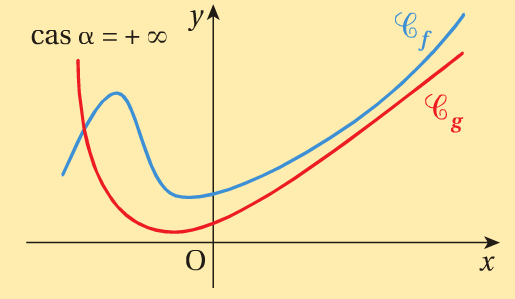
\includegraphics[width=0.8\textwidth]{comp1.png}
\caption{Courbe de (Cf)}
\label{fig:monimage}
\end{figure}

Si:
       \begin{itemize}
       \item Pour tout \( x\in I \) \( f(x)\leq g(x) \) 
        \item \( \lim_{x \to \alpha}g(x)=-\infty \)
       \end{itemize}
Alors \( \lim_{x \to \alpha}f(x)=-\infty \)
   
\begin{figure}[H]% Forcer l'image à cet endroit
\centering
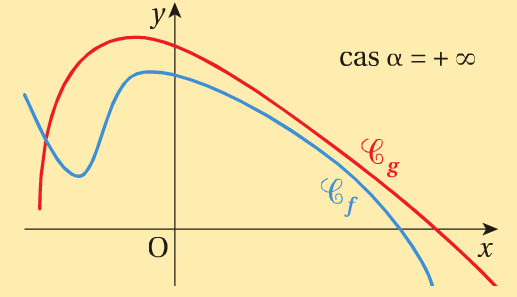
\includegraphics[width=0.8\textwidth]{comp2.png}
\caption{Courbe de (Cf)}
\label{fig:monimage}
\end{figure}

       	\textbf{\underline{Exemple 1}}
       	\[ \text{Soit \( f(x)=-x+\sin x \) Calculer }\lim_{x \to +\infty} f(x) \]
       	\textbf{\underline{Solution}}
       	\[ \text{Posons \( g(x)=-x+1 \) Comme, pour tout \(x\), \(\sin x\leq 1\), on a, pour tout \(x\), \( f(x)\leq g(x) \).} \]
       	\[ \text{Or,} \lim_{x \to +\infty}g(x)=-\infty, \text{donc} \lim_{x \to +\infty}f(x)=-\infty\]       	
       	
       	 \textbf{\underline{Exemple 2}}
       	\[ \text{Soit \( g(x)=\frac{\sqrt{1+x^{2}}}{x^{2}} \). Calculer }\lim_{x \to 0} g(x) \]
       	\textbf{\underline{Solution}}
       	 \[ \text{Posons \( f(x)=\frac{1}{x^{2}} \). Comme, pour tout \(x\neq 0\), on a, \( 1\leq \sqrt{1+x^{2}} \)., on a, pour tout }, x\neq 0 \]
       	\[ f(x)\geq g(x) \text{ Or,} \lim_{x \to 0}g(x)=+\infty, \text{donc} \lim_{x \to 0}f(x)=+\infty\]
       	
       	\item \textcolor{green}{\underline{Théorème d’encadrement ou théorème des gendarmes}}
       	
Soient \( f \), \( g \) et \( h \) trois fonctions définies sur un intervalle \( I \) au voisianage \( \alpha \), \( \alpha \) étant un réel, \( +\infty \) ou \( -\infty \).

Si \( \forall x\in I \quad g(x) \leq f(x)\leq h(x) \) et \( \lim_{x \to \alpha}g(x)=\lim_{x \to \alpha}h(x)=\ell,\) alors \( \lim_{x \to \alpha}f(x)=\ell \)
       	
       	\textbf{\underline{Exercice d'application}}
\[\text{ Calculer } \lim_{ x\to +\infty} \frac{x-\sin x}{x^{2}} \]   	
       	\textbf{\underline{Solution}}
       	
      	
			       		
 %      	\textbf{\underline{Exercice d'application}}
       	
 %      	\textbf{Remarque}
       	
%       	\textbf{\underline{Exercice d'application}}
\end{enumerate}
%		\item \textbf{\textcolor{blue}{\underline{Interprétations gémétriques des limites}}}
		
%		\begin{enumerate}[label=\alph*)]
%		\item \textcolor{green}{\underline{Asymptote horizontale (AH) ou asymptote parllèle à \( (ox) \)}}
		
%		\item \textcolor{green}{\underline{Asymptote verticale (AV) ou asymptote parllèle à \( (oy) \)}}
		
%		\item \textcolor{green}{\underline{Asymptote oblique (AO)}}
		
%		\textbf{Propriété 1}
		
%		\textbf{Remarque}
		
%		\textbf{Propriété 2}
		
%		\textbf{\underline{Exercice d'application}}
		
%		\item \textcolor{green}{\underline{Branche parabolique de direction (oy)}}

%		\textbf{Remarque}		
		
%		\item \textcolor{green}{\underline{Branche pparabolique de direction (ox)}}

%		\textbf{Remarque}			
		
%		\item \textcolor{green}{\underline{Branche parabolique de direction y = ax}}
		
%		\textbf{Remarque}	
		
%		\item \textcolor{green}{\underline{Définition}}
		
%		\textbf{\underline{Exercice d'application}}
%		\end{enumerate}
		
\end{enumerate}

%\subsection*{\underline{\textbf{\textcolor{red}{II.Continuité}}}}

%\begin{enumerate}[label=\arabic*)]
%\item \textbf{\textcolor{blue}{\underline{Définition}}}

%			\textbf{\underline{Exercice d'application}}
			
%			\textbf{\underline{Solution}}
			
%\item \textbf{\textcolor{blue}{\underline{Continuité à gauche et continuité à droite}}}

%			\textbf{\underline{Exercice d'application}}
			
%			\textbf{\underline{Solution}}

%\item \textbf{\textcolor{blue}{\underline{Prolongement par continuité}}}	

%			\textbf{\underline{Exercice d'application}}
			
%			\textbf{\underline{Solution}}	
			
%\item \textbf{\textcolor{blue}{\underline{Continuité sur un intervalle}}}

%\item \textbf{\textcolor{blue}{\underline{Continuité de fonctions usuelles}}}

%\textbf{\underline{Propriété}}

%\item \textbf{\textcolor{blue}{\underline{Opérations sur les fonctions continues}}}

%\item \textbf{\textcolor{blue}{\underline{Compositions de deux fonctions continues}}}

%\item \textbf{\textcolor{blue}{\underline{Continuité à gauche et continuité à droite}}}

%			\textbf{\underline{Exercice d'application}}
			
%			\textbf{\underline{Solution}}

%\item \textbf{\textcolor{blue}{\underline{Propriété des fonctions continues sur un intervalle}}}

%			\textbf{\underline{Théorème}}

%\item \textbf{\textcolor{blue}{\underline{Image d’unintervalle par une fonction continue et stritement monotone}}}

%			\textbf{\underline{Exercice d'application}}
			
%			\textbf{\underline{Solution}}

%\item \textbf{\textcolor{blue}{\underline{Théorème des valeurs intermediaries}}}

%			\textbf{\underline{Exercice d'application}}
			
%			\textbf{\underline{Solution}}

%\item \textbf{\textcolor{blue}{\underline{Théorème d’existence d’une bijection}}}

%			\textbf{\underline{Exercice d'application}}
			
%			\textbf{\underline{Solution}}

%\item \textbf{\textcolor{blue}{\underline{Théorème d’existence et d’unicité d’une solution}}}

%			\textbf{\underline{Exercice d'application}}
			
%			\textbf{\underline{Solution}}

%\item \textbf{\textcolor{blue}{\underline{Encadrement de la racine \( \alpha \) à \( \epsilon \) près}}}

%			\textbf{\underline{Méthode de balayage(Approche par exemple)}}

%			\textbf{\underline{Solution}}			

%			\textbf{\underline{Exercice d'application}}
			
%			\textbf{\underline{Solution}}			
			
%\item \textbf{\textcolor{blue}{\underline{Calcul de \( f^{-1}(y_{0}) \) sans connaître l'expression \( f^{-1} \) }}}

			%\textbf{\underline{Exercice d'application}}
			
			%\textbf{\underline{Solution}}	

%\item \textbf{\textcolor{blue}{\underline{Expression de \( f^{-1} \) }}}

			%\textbf{\underline{Exercice d'application}}
			
			%\textbf{\underline{Solution}}

%\item \textbf{\textcolor{blue}{\underline{Bijection réciproque d’une fonction continue et steictement monotone }}}

%\end{enumerate}

%\section*{\underline{\textbf{\textcolor{red}{B. DÉRIVATION ET ÉTUDES DE FONCTIONS}}}}
\end{document}
